\documentclass[final,10pt,times,twocolumn]{elsarticle}
\usepackage[top = 4cm, bottom = 3cm, right = 2cm, left = 2cm, a4paper]{geometry}
\usepackage{amssymb}
\usepackage[backref]{hyperref}
\hypersetup{
    colorlinks=true,
    linkcolor=blue,
    filecolor=magenta,      
    urlcolor=cyan,
    pdftitle={Overleaf Example},
    pdfpagemode=FullScreen,
    }
\usepackage{color}
\author{Jhih-Jia Hung}

\begin{document}
\begin{frontmatter}
\title{Uranium diboride, the potential candidates of ATF, feature and application \\ \LaTeX}
\begin{abstract}
It is universally acknowledged that power generation is most fundamental facility required by every industry, as almost all things require electricity to work. Among all the methods of electricity generation, nuclear power always faces considerable scrutiny. Undoubtedly, nuclear power brings about feelings of fear and unknown horror, especially after the accidents at Fukushima and Chernobyl. Such concerns are not unreasonable, as people's fear of nuclear power is a good measure to prevent accidents from happening. However, Taiwan people are too afraid of using this technology, turns out the result is miss out the opportunity to improve our ecosystem and make it more environmentally friendly. In this research, I would put the focus on the potentially fuel, Uranium diboride (UB$_{2}$), an interesting fuel that nowadays are research to be an ATF candidate fuel. Its physical properties also make it suitable for use in GEN-IV reactors, which require high standards to reaction. All of these factors make UB$_{2}$ show on my eyes, and this research aims to explore its potential.
\end{abstract}

\begin{keyword}
ATF, Uranium diboride, GEN-IV reactors
\end{keyword}

\end{frontmatter}

\section{Introduction}
Uranium diboride is potentially material which on closely debating to be the next generation reactors fuel, expecialy known as ATFs( Advanced Technology Fuels or Accident Tolerance Fuels ). UB2 have unique talent that play a important role in. And ATFs is aim to increase the reactors power up-rates, longer cycle lengths, improved performance,and reduced stored energy in the core etc. And allow have more time to coping during accident scenarios.\cite{watkins2022challenges}

\begin{figure}[ht]
    \centering
    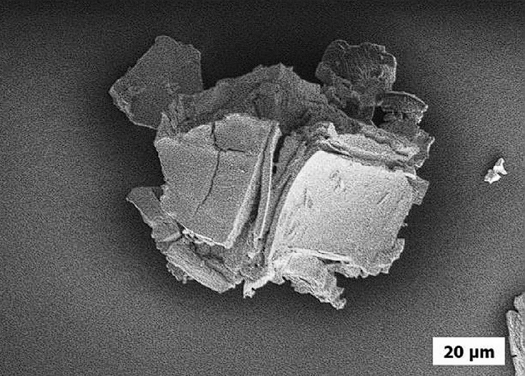
\includegraphics[width = 5.75cm]{UB2 Micrographs.png}
    \caption{UB2 Micrographs Picture\cite{watkins2022challenges} }
\end{figure}

\section{Physical properties}
In many candidate of ATFs material, the Uranium diboride has higher Uranium density than the others. Also, it has better thermal conductive that make itself have lower fuel centre-line temperatures on working, result in many positive effect such like; reduce the rate of temperature-dependent release of fission products, reduce the energy stored inside the fuel (This properties also is the most important that the UB2 need.)

\bibliographystyle{IEEEtran}
\bibliography{sample}

\end{document}
\endinput